\documentclass{article}
\usepackage[T1]{fontenc}
\usepackage{lmodern}
\usepackage{cite}
\usepackage{amsmath,amssymb,amsfonts}
\usepackage{graphicx}
\usepackage{textcomp}
\usepackage{xcolor}
\usepackage{url}
\usepackage{microtype}
\usepackage{tikz}
\usetikzlibrary{arrows.meta,positioning}
\usepackage[left=3cm,right=3cm,top=2cm,bottom=2cm]{geometry}
\setlength{\parskip}{0.4em}

\begin{document}
\title{ATAI Evaluation Event IV\\[0.3em]
\large \textit{TitaniumTwinklingSnake}}
\author{Tristan Hein (\textit{h159}) \and Thi Tho Pham (\textit{h152})}
\date{}
\maketitle

\section{Agent Overview and Capabilities}
Our agent helps users choose a movie through a short conversation. Rather than
immediately listing titles, it asks what the user enjoyed or wants next, such as
a similar mood, a particular release period, or more films by the same director.
It remembers the answer and combines it with the preferences already supplied.
When enough information is available, it recommends films from the course
knowledge graph, with release years and brief reasons for each choice.

The main addition for Evaluation IV is this preference-gathering dialogue.
The agent understands short replies such as ``2010s'' and ``same director'',
handles corrections, and avoids repeating liked, seen, or previously suggested
films. A new standalone request starts a fresh search. The factual question
answering and safety routing from Stage 3 remain available without interrupting
the active recommendation context.

\section{Adopted Methods}
\begin{itemize}
\setlength{\itemsep}{0pt}
\item \textbf{Language understanding.} We use local
\texttt{Qwen/Qwen3.5-4B}~\cite{qwen35} through vLLM~\cite{vllm}, with greedy
decoding and thinking output disabled. One prompt classifies the current turn
and identifies its action; a focused extraction prompt captures preference
changes. Python validates the returned fields before updating memory.

\item \textbf{Conversation state.} Each room/user pair has its own preferences,
pending question, recent history, and suggested-film IDs. Shared graph features
help formulate a relevant clarification, but are not treated as confirmed
preferences. Readiness is interpreted in the context of the pending question.

\item \textbf{Graph retrieval.} PyOxigraph~\cite{pyoxigraph} loads the supplied
RDF graph. Labels, aliases, and conservative fuzzy matching resolve film names.
Factual filters enforce genre, people, country, language, release years, awards,
and ratings. A weighted score favors shared features, especially costume design
and direction. Mood/content requests can trigger model selection from a bounded
candidate list; only retrieved IDs are accepted.

\item \textbf{Response generation.} Qwen asks one focused question or explains
the selected films using supplied graph evidence. Structured outputs constrain
the format. Unsupported filters, such as streaming availability, require
clarification rather than an invented guarantee.
\end{itemize}

\section{Pipeline}
The flow below separates conversational interpretation from factual retrieval.
Blocked requests leave the pipeline after classification; independent factual
questions use the inherited query handler.

\begin{center}
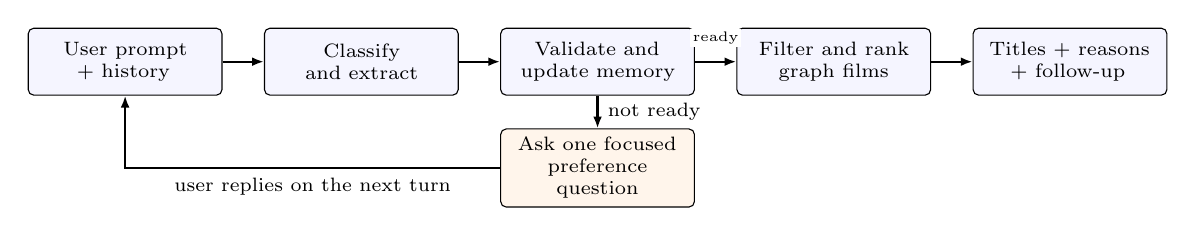
\begin{tikzpicture}[
  font=\scriptsize,
  box/.style={draw,rounded corners=2pt,align=center,text width=2.25cm,
              minimum height=0.85cm,inner sep=3pt,fill=blue!4},
  arrow/.style={-{Latex[length=1.5mm]},thick}
]
\node[box] (input) at (0,0) {User prompt\\+ history};
\node[box] (route) at (3,0) {Classify\\and extract};
\node[box] (state) at (6,0) {Validate and\\update memory};
\node[box] (retrieve) at (9,0) {Filter and rank\\graph films};
\node[box] (answer) at (12,0) {Titles + reasons\\+ follow-up};
\node[box,fill=orange!8] (ask) at (6,-1.35) {Ask one focused\\preference question};
\draw[arrow] (input) -- (route);
\draw[arrow] (route) -- (state);
\draw[arrow] (state) -- node[above=5pt,font=\tiny,fill=white,inner sep=1pt] {ready} (retrieve);
\draw[arrow] (retrieve) -- (answer);
\draw[arrow] (state) -- node[right] {not ready} (ask);
\draw[arrow] (ask.west) -| node[pos=0.25,below] {user replies on the next turn} (input.south);
\end{tikzpicture}
\end{center}

One saved live conversation~\cite{live} starts with: ``I enjoyed The Handmaiden
and Decision to Leave. What else do you recommend?'' The router identifies a safe
recommendation request and extracts both liked titles. Graph lookup finds their
shared director, Park Chan-wook. Instead of assuming that this is the user's
reason for liking them, the agent asks: ``Since both films are by Park Chan-wook,
do you want more of his work, or are you looking for similar movies from other
directors?''

The user replies: ``More South Korean thrillers by the same director,
Park Chan-wook. Three please.'' The profile contains
\texttt{focus=director}, \texttt{genres=[thriller film]},
\texttt{countries=[South Korea]}, and \texttt{count=3}. Retrieval requires
the shared director, requested genre and country, and excludes the two seeds.
It returns \emph{Oldboy} (2003), \emph{Sympathy for Lady Vengeance} (2005), and
\emph{Sympathy for Mr.\ Vengeance} (2002), followed by brief reasons and an offer
to continue. The graph checks confirm that these satisfy the requested facets.
This is an earlier live trace, not a new run of the latest wording prompts;
graph correctness alone does not establish how much the user will enjoy them.

\section{Improvements}
During development, a new request could be interpreted as an answer to an older
question, allowing unrelated preferences to affect the search. We moved
new-search detection ahead of focused extraction, so a standalone request with
new liked titles receives a fresh profile. Explicit additions still extend the
existing search. We also corrected title matching: extracted, unquoted names
now receive conservative typo matching, so ``Interstelar'' resolves to
\emph{Interstellar}; ambiguous remakes still require a year.

To match Evaluation IV, clarification is now the default rather than immediate
recommendation. The wording prompts favor a short, relevant question and concise
reasons tied to the user's answer. Ordinary safe replies omit internal labels.
All 118 current automated tests pass, including first-turn clarification,
reply handling, title typos, search isolation, exclusions, and safety. These
tests use controlled model responses, so naturalness still needs human review.

\section{Additional Features}
The local API supports isolated sessions, explicit resets, and reproducible
evaluation without contacting Speakeasy. An earlier live run passed 64/64 checks
across 21 turns~\cite{live}; a broader conversation suite passed 13/15 cases
(161/174 checks)~\cite{suite}. The remaining cases involved combined constraints
and dropping unsupported filters. These are development results from earlier
revisions, not an official Evaluation IV score or validation of the latest
wording. Generated reasons are evidence-constrained, but are not independently
checked for factual entailment.

% The course permits references beyond the two-page main-report limit.
\clearpage
\bibliographystyle{abbrv}
\bibliography{references}
\end{document}
